% Figure 1 — deployed pipeline schematic (standalone, auto-cropped vector PDF).
% Compile: pdflatex figure1_pipeline.tex  ->  figure1_pipeline.pdf
\documentclass[border=2pt]{standalone}
\usepackage{mathptmx}
\usepackage{amsmath,amssymb}
\usepackage{tikz}
\usepackage{pgfplots}
\pgfplotsset{compat=1.17}
\usetikzlibrary{arrows.meta,positioning,calc,shapes.geometric,fit,backgrounds}
\newcommand{\Pup}{\hat p}
\newcommand{\ece}{\mathrm{ECE}}
\begin{document}
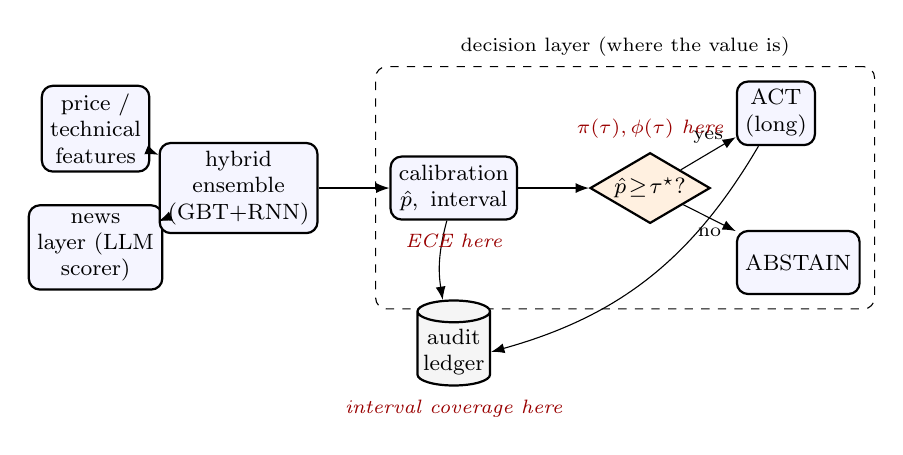
\begin{tikzpicture}[
  font=\footnotesize,
  box/.style={rectangle,rounded corners,draw,thick,align=center,inner sep=3pt,minimum height=8mm,fill=blue!4},
  gate/.style={diamond,draw,thick,align=center,inner sep=1pt,aspect=1.7,fill=orange!12},
  store/.style={cylinder,shape border rotate=90,aspect=0.3,draw,thick,align=center,inner sep=2pt,fill=gray!8},
  meas/.style={font=\scriptsize\itshape,red!60!black},
  >=Latex
]
\node[box] (px) {price /\\technical\\features};
\node[box,below=4mm of px] (news) {news\\layer (LLM\\scorer)};
\node[box,right=8mm of $(px)!0.5!(news)$] (ens) {hybrid\\ensemble\\(GBT+RNN)};
\node[box,right=9mm of ens] (cal) {calibration\\$\Pup,\ \text{interval}$};
\node[gate,right=9mm of cal] (g) {$\Pup\!\ge\!\tau^\star$?};
\node[box,above right=3mm and 7mm of g] (act) {ACT\\(long)};
\node[box,below right=3mm and 7mm of g] (ab) {ABSTAIN};
\node[store,below=10mm of cal] (led) {audit\\ledger};
\draw[->] (px)--(ens); \draw[->] (news)--(ens);
\draw[->] (ens)--(cal); \draw[->] (cal)--(g);
\draw[->] (g)-- node[above,font=\scriptsize]{yes} (act);
\draw[->] (g)-- node[below,font=\scriptsize]{no} (ab);
\draw[->] (cal) to[bend right=12] (led);
\draw[->] (act) to[bend left=22] (led.east);
\node[meas,below=0.5mm of cal] {ECE here};
\node[meas,above=0.5mm of g] {$\pi(\tau),\phi(\tau)$ here};
\node[meas,below=0.5mm of led] {interval coverage here};
\begin{scope}[on background layer]
\node[draw,dashed,rounded corners,fit=(cal)(g)(act)(ab),inner sep=5pt,label=above:{\scriptsize decision layer (where the value is)}] {};
\end{scope}
\end{tikzpicture}
\end{document}
